\documentclass[1p]{elsarticle_modified}
%\bibliographystyle{elsarticle-num}

%\usepackage[colorlinks]{hyperref}
%\usepackage{abbrmath_seonhwa} %\Abb, \Ascr, \Acal ,\Abf, \Afrak
\usepackage{amsfonts}
\usepackage{amssymb}
\usepackage{amsmath}
\usepackage{amsthm}
\usepackage{scalefnt}
\usepackage{amsbsy}
\usepackage{kotex}
\usepackage{caption}
\usepackage{subfig}
\usepackage{color}
\usepackage{graphicx}
\usepackage{xcolor} %% white, black, red, green, blue, cyan, magenta, yellow
\usepackage{float}
\usepackage{setspace}
\usepackage{hyperref}

\usepackage{tikz}
\usetikzlibrary{arrows}

\usepackage{multirow}
\usepackage{array} % fixed length table
\usepackage{hhline}

%%%%%%%%%%%%%%%%%%%%%
\makeatletter
\renewcommand*\env@matrix[1][\arraystretch]{%
	\edef\arraystretch{#1}%
	\hskip -\arraycolsep
	\let\@ifnextchar\new@ifnextchar
	\array{*\c@MaxMatrixCols c}}
\makeatother %https://tex.stackexchange.com/questions/14071/how-can-i-increase-the-line-spacing-in-a-matrix
%%%%%%%%%%%%%%%

\usepackage[normalem]{ulem}

\newcommand{\msout}[1]{\ifmmode\text{\sout{\ensuremath{#1}}}\else\sout{#1}\fi}
%SOURCE: \msout is \stkout macro in https://tex.stackexchange.com/questions/20609/strikeout-in-math-mode

\newcommand{\cancel}[1]{
	\ifmmode
	{\color{red}\msout{#1}}
	\else
	{\color{red}\sout{#1}}
	\fi
}

\newcommand{\add}[1]{
	{\color{blue}\uwave{#1}}
}

\newcommand{\replace}[2]{
	\ifmmode
	{\color{red}\msout{#1}}{\color{blue}\uwave{#2}}
	\else
	{\color{red}\sout{#1}}{\color{blue}\uwave{#2}}
	\fi
}

\newcommand{\Sol}{\mathcal{S}} %segment
\newcommand{\D}{D} %diagram
\newcommand{\A}{\mathcal{A}} %arc


%%%%%%%%%%%%%%%%%%%%%%%%%%%%%5 test

\def\sl{\operatorname{\textup{SL}}(2,\Cbb)}
\def\psl{\operatorname{\textup{PSL}}(2,\Cbb)}
\def\quan{\mkern 1mu \triangleright \mkern 1mu}

\theoremstyle{definition}
\newtheorem{thm}{Theorem}[section]
\newtheorem{prop}[thm]{Proposition}
\newtheorem{lem}[thm]{Lemma}
\newtheorem{ques}[thm]{Question}
\newtheorem{cor}[thm]{Corollary}
\newtheorem{defn}[thm]{Definition}
\newtheorem{exam}[thm]{Example}
\newtheorem{rmk}[thm]{Remark}
\newtheorem{alg}[thm]{Algorithm}

\newcommand{\I}{\sqrt{-1}}
\begin{document}

%\begin{frontmatter}
%
%\title{Boundary parabolic representations of knots up to 8 crossings}
%
%%% Group authors per affiliation:
%\author{Yunhi Cho} 
%\address{Department of Mathematics, University of Seoul, Seoul, Korea}
%\ead{yhcho@uos.ac.kr}
%
%
%\author{Seonhwa Kim} %\fnref{s_kim}}
%\address{Center for Geometry and Physics, Institute for Basic Science, Pohang, 37673, Korea}
%\ead{ryeona17@ibs.re.kr}
%
%\author{Hyuk Kim}
%\address{Department of Mathematical Sciences, Seoul National University, Seoul 08826, Korea}
%\ead{hyukkim@snu.ac.kr}
%
%\author{Seokbeom Yoon}
%\address{Department of Mathematical Sciences, Seoul National University, Seoul, 08826,  Korea}
%\ead{sbyoon15@snu.ac.kr}
%
%\begin{abstract}
%We find all boundary parabolic representation of knots up to 8 crossings.
%
%\end{abstract}
%\begin{keyword}
%    \MSC[2010] 57M25 
%\end{keyword}
%
%\end{frontmatter}

%\linenumbers
%\tableofcontents
%
\newcommand\colored[1]{\textcolor{white}{\rule[-0.35ex]{0.8em}{1.4ex}}\kern-0.8em\color{red} #1}%
%\newcommand\colored[1]{\textcolor{white}{ #1}\kern-2.17ex	\textcolor{white}{ #1}\kern-1.81ex	\textcolor{white}{ #1}\kern-2.15ex\color{red}#1	}

{\Large $\underline{12a_{0767}~(K12a_{0767})}$}

\setlength{\tabcolsep}{10pt}
\renewcommand{\arraystretch}{1.6}
\vspace{1cm}\begin{tabular}{m{100pt}>{\centering\arraybackslash}m{274pt}}
\multirow{5}{120pt}{
	\centering
	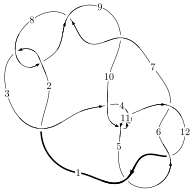
\includegraphics[width=112pt]{../../../GIT/diagram.site/Diagrams/png/1568_12a_0767.png}\\
\ \ \ A knot diagram\footnotemark}&
\allowdisplaybreaks
\textbf{Linearized knot diagam} \\
\cline{2-2}
 &
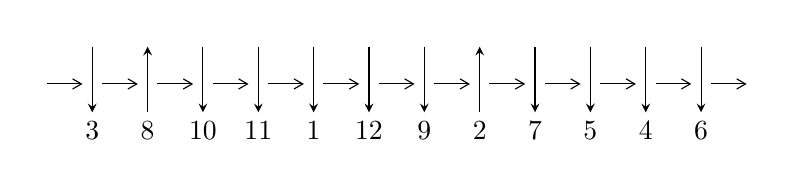
\begin{tikzpicture}[x=20pt, y=17pt]
	% nodes
	\node (C0) at (0, 0) {};
	\node (C1) at (1, 0) {};
	\node (C1U) at (1, +1) {};
	\node (C1D) at (1, -1) {3};

	\node (C2) at (2, 0) {};
	\node (C2U) at (2, +1) {};
	\node (C2D) at (2, -1) {8};

	\node (C3) at (3, 0) {};
	\node (C3U) at (3, +1) {};
	\node (C3D) at (3, -1) {10};

	\node (C4) at (4, 0) {};
	\node (C4U) at (4, +1) {};
	\node (C4D) at (4, -1) {11};

	\node (C5) at (5, 0) {};
	\node (C5U) at (5, +1) {};
	\node (C5D) at (5, -1) {1};

	\node (C6) at (6, 0) {};
	\node (C6U) at (6, +1) {};
	\node (C6D) at (6, -1) {12};

	\node (C7) at (7, 0) {};
	\node (C7U) at (7, +1) {};
	\node (C7D) at (7, -1) {9};

	\node (C8) at (8, 0) {};
	\node (C8U) at (8, +1) {};
	\node (C8D) at (8, -1) {2};

	\node (C9) at (9, 0) {};
	\node (C9U) at (9, +1) {};
	\node (C9D) at (9, -1) {7};

	\node (C10) at (10, 0) {};
	\node (C10U) at (10, +1) {};
	\node (C10D) at (10, -1) {5};

	\node (C11) at (11, 0) {};
	\node (C11U) at (11, +1) {};
	\node (C11D) at (11, -1) {4};

	\node (C12) at (12, 0) {};
	\node (C12U) at (12, +1) {};
	\node (C12D) at (12, -1) {6};
	\node (C13) at (13, 0) {};

	% arrows
	\draw[->,>={angle 60}]
	(C0) edge (C1) (C1) edge (C2) (C2) edge (C3) (C3) edge (C4) (C4) edge (C5) (C5) edge (C6) (C6) edge (C7) (C7) edge (C8) (C8) edge (C9) (C9) edge (C10) (C10) edge (C11) (C11) edge (C12) (C12) edge (C13) ;	\draw[->,>=stealth]
	(C1U) edge (C1D) (C2D) edge (C2U) (C3U) edge (C3D) (C4U) edge (C4D) (C5U) edge (C5D) (C6U) edge (C6D) (C7U) edge (C7D) (C8D) edge (C8U) (C9U) edge (C9D) (C10U) edge (C10D) (C11U) edge (C11D) (C12U) edge (C12D) ;
	\end{tikzpicture} \\
\hhline{~~} \\& 
\textbf{Solving Sequence} \\ \cline{2-2} 
 &
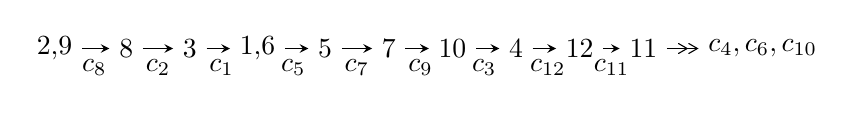
\begin{tikzpicture}[x=23pt, y=7pt]
	% node
	\node (A0) at (-1/8, 0) {2,9};
	\node (A1) at (1, 0) {8};
	\node (A2) at (2, 0) {3};
	\node (A3) at (49/16, 0) {1,6};
	\node (A4) at (33/8, 0) {5};
	\node (A5) at (41/8, 0) {7};
	\node (A6) at (49/8, 0) {10};
	\node (A7) at (57/8, 0) {4};
	\node (A8) at (65/8, 0) {12};
	\node (A9) at (73/8, 0) {11};
	\node (C1) at (1/2, -1) {$c_{8}$};
	\node (C2) at (3/2, -1) {$c_{2}$};
	\node (C3) at (5/2, -1) {$c_{1}$};
	\node (C4) at (29/8, -1) {$c_{5}$};
	\node (C5) at (37/8, -1) {$c_{7}$};
	\node (C6) at (45/8, -1) {$c_{9}$};
	\node (C7) at (53/8, -1) {$c_{3}$};
	\node (C8) at (61/8, -1) {$c_{12}$};
	\node (C9) at (69/8, -1) {$c_{11}$};
	\node (A10) at (11, 0) {$c_{4},c_{6},c_{10}$};

	% edge
	\draw[->,>=stealth]	
	(A0) edge (A1) (A1) edge (A2) (A2) edge (A3) (A3) edge (A4) (A4) edge (A5) (A5) edge (A6) (A6) edge (A7) (A7) edge (A8) (A8) edge (A9) ;
	\draw[->>,>={angle 60}]	
	(A9) edge (A10);
\end{tikzpicture} \\ 

\end{tabular} \\

\footnotetext{
The image of knot diagram is generated by the software ``\textbf{Draw programme}" developed by Andrew Bartholomew(\url{http://www.layer8.co.uk/maths/draw/index.htm\#Running-draw}), where we modified some parts for our purpose(\url{https://github.com/CATsTAILs/LinksPainter}).
}\phantom \\ \newline 
\centering \textbf{Ideals for irreducible components\footnotemark of $X_{\text{par}}$} 
 
\begin{align*}
I^u_{1}&=\langle 
2 u^{25}+3 u^{24}+\cdots+b-3,\;3 u^{26}+9 u^{25}+\cdots+2 a-9,\;u^{27}+3 u^{26}+\cdots+u-2\rangle \\
I^u_{2}&=\langle 
21 u^{19} a+223 u^{19}+\cdots-81 a-318,\;-2 u^{19} a+u^{19}+\cdots+a^2-3,\;u^{20}- u^{19}+\cdots+u^2+1\rangle \\
I^u_{3}&=\langle 
- u^5+b- u,\;- u^4- u^2+a+u-2,\;u^6+u^4+2 u^2+1\rangle \\
\\
\end{align*}
\raggedright * 3 irreducible components of $\dim_{\mathbb{C}}=0$, with total 73 representations.\\
\footnotetext{All coefficients of polynomials are rational numbers. But the coefficients are sometimes approximated in decimal forms when there is not enough margin.}
\newpage
\renewcommand{\arraystretch}{1}
\centering \section*{I. $I^u_{1}= \langle 2 u^{25}+3 u^{24}+\cdots+b-3,\;3 u^{26}+9 u^{25}+\cdots+2 a-9,\;u^{27}+3 u^{26}+\cdots+u-2 \rangle$}
\flushleft \textbf{(i) Arc colorings}\\
\begin{tabular}{m{7pt} m{180pt} m{7pt} m{180pt} }
\flushright $a_{2}=$&$\begin{pmatrix}0\\u\end{pmatrix}$ \\
\flushright $a_{9}=$&$\begin{pmatrix}1\\0\end{pmatrix}$ \\
\flushright $a_{8}=$&$\begin{pmatrix}1\\u^2\end{pmatrix}$ \\
\flushright $a_{3}=$&$\begin{pmatrix}u\\u^3+u\end{pmatrix}$ \\
\flushright $a_{1}=$&$\begin{pmatrix}u^3\\u^5+u^3+u\end{pmatrix}$ \\
\flushright $a_{6}=$&$\begin{pmatrix}-\frac{3}{2} u^{26}-\frac{9}{2} u^{25}+\cdots-4 u+\frac{9}{2}\\-2 u^{25}-3 u^{24}+\cdots-5 u+3\end{pmatrix}$ \\
\flushright $a_{5}=$&$\begin{pmatrix}-\frac{7}{2} u^{26}-\frac{21}{2} u^{25}+\cdots-8 u+\frac{17}{2}\\-5 u^{25}-7 u^{24}+\cdots-12 u+7\end{pmatrix}$ \\
\flushright $a_{7}=$&$\begin{pmatrix}u^2+1\\u^2\end{pmatrix}$ \\
\flushright $a_{10}=$&$\begin{pmatrix}u^4+u^2+1\\u^4\end{pmatrix}$ \\
\flushright $a_{4}=$&$\begin{pmatrix}- u^{11}-2 u^9-4 u^7-4 u^5-3 u^3\\- u^{11}- u^9-2 u^7- u^5+u^3+u\end{pmatrix}$ \\
\flushright $a_{12}=$&$\begin{pmatrix}-\frac{3}{2} u^{26}-\frac{5}{2} u^{25}+\cdots+2 u+\frac{1}{2}\\- u^{26}-2 u^{25}+\cdots+u+1\end{pmatrix}$ \\
\flushright $a_{11}=$&$\begin{pmatrix}\frac{1}{2} u^{26}+\frac{1}{2} u^{25}+\cdots+\frac{1}{2} u^2+\frac{1}{2}\\u^{26}+2 u^{25}+\cdots+u-1\end{pmatrix}$\\&\end{tabular}
\flushleft \textbf{(ii) Obstruction class $= -1$}\\~\\
\flushleft \textbf{(iii) Cusp Shapes $= -4 u^{26}-10 u^{25}-26 u^{24}-38 u^{23}-78 u^{22}-106 u^{21}-180 u^{20}-202 u^{19}-298 u^{18}-286 u^{17}-366 u^{16}-274 u^{15}-332 u^{14}-172 u^{13}-200 u^{12}-10 u^{11}-70 u^{10}+84 u^9-18 u^8+58 u^7-62 u^6+10 u^5-52 u^4+6 u^3-18 u^2+14 u-10$}\\~\\
\newpage\renewcommand{\arraystretch}{1}
\flushleft \textbf{(iv) u-Polynomials at the component}\newline \\
\begin{tabular}{m{50pt}|m{274pt}}
Crossings & \hspace{64pt}u-Polynomials at each crossing \\
\hline $$\begin{aligned}c_{1},c_{7},c_{9}\end{aligned}$$&$\begin{aligned}
&u^{27}+7 u^{26}+\cdots-7 u-4
\end{aligned}$\\
\hline $$\begin{aligned}c_{2},c_{8}\end{aligned}$$&$\begin{aligned}
&u^{27}-3 u^{26}+\cdots+u+2
\end{aligned}$\\
\hline $$\begin{aligned}c_{3}\end{aligned}$$&$\begin{aligned}
&u^{27}-3 u^{26}+\cdots+192 u+128
\end{aligned}$\\
\hline $$\begin{aligned}c_{4},c_{5},c_{6}\\c_{10},c_{11},c_{12}\end{aligned}$$&$\begin{aligned}
&u^{27}+15 u^{25}+\cdots+3 u+1
\end{aligned}$\\
\hline
\end{tabular}\\~\\
\newpage\renewcommand{\arraystretch}{1}
\flushleft \textbf{(v) Riley Polynomials at the component}\newline \\
\begin{tabular}{m{50pt}|m{274pt}}
Crossings & \hspace{64pt}Riley Polynomials at each crossing \\
\hline $$\begin{aligned}c_{1},c_{7},c_{9}\end{aligned}$$&$\begin{aligned}
&y^{27}+27 y^{26}+\cdots+385 y-16
\end{aligned}$\\
\hline $$\begin{aligned}c_{2},c_{8}\end{aligned}$$&$\begin{aligned}
&y^{27}+7 y^{26}+\cdots-7 y-4
\end{aligned}$\\
\hline $$\begin{aligned}c_{3}\end{aligned}$$&$\begin{aligned}
&y^{27}+y^{26}+\cdots-323584 y-16384
\end{aligned}$\\
\hline $$\begin{aligned}c_{4},c_{5},c_{6}\\c_{10},c_{11},c_{12}\end{aligned}$$&$\begin{aligned}
&y^{27}+30 y^{26}+\cdots-7 y-1
\end{aligned}$\\
\hline
\end{tabular}\\~\\
\newpage\flushleft \textbf{(vi) Complex Volumes and Cusp Shapes}
$$\begin{array}{c|c|c}  
\text{Solutions to }I^u_{1}& \I (\text{vol} + \sqrt{-1}CS) & \text{Cusp shape}\\
 \hline 
\begin{aligned}
u &= \phantom{-}0.277460 + 0.929850 I \\
a &= -0.226509 + 0.100294 I \\
b &= -0.350781 + 0.505562 I\end{aligned}
 & -3.57952 + 2.60716 I & -14.9352 - 5.3810 I \\ \hline\begin{aligned}
u &= \phantom{-}0.277460 - 0.929850 I \\
a &= -0.226509 - 0.100294 I \\
b &= -0.350781 - 0.505562 I\end{aligned}
 & -3.57952 - 2.60716 I & -14.9352 + 5.3810 I \\ \hline\begin{aligned}
u &= \phantom{-}0.126747 + 1.039010 I \\
a &= \phantom{-}1.75601 + 0.00499 I \\
b &= -0.485752 + 0.316127 I\end{aligned}
 & \phantom{-}4.48046 - 3.61631 I & -5.50483 + 2.14074 I \\ \hline\begin{aligned}
u &= \phantom{-}0.126747 - 1.039010 I \\
a &= \phantom{-}1.75601 - 0.00499 I \\
b &= -0.485752 - 0.316127 I\end{aligned}
 & \phantom{-}4.48046 + 3.61631 I & -5.50483 - 2.14074 I \\ \hline\begin{aligned}
u &= -0.752094 + 0.565194 I \\
a &= -0.248696 + 0.216030 I \\
b &= \phantom{-}1.22743 + 0.73470 I\end{aligned}
 & \phantom{-}10.36450 - 3.20982 I & \phantom{-}1.89568 + 3.18066 I \\ \hline\begin{aligned}
u &= -0.752094 - 0.565194 I \\
a &= -0.248696 - 0.216030 I \\
b &= \phantom{-}1.22743 - 0.73470 I\end{aligned}
 & \phantom{-}10.36450 + 3.20982 I & \phantom{-}1.89568 - 3.18066 I \\ \hline\begin{aligned}
u &= \phantom{-}0.387921 + 1.022180 I \\
a &= -0.396664 + 1.123690 I \\
b &= -0.35306 - 1.73889 I\end{aligned}
 & \phantom{-}6.03730 + 9.94630 I & -4.12408 - 8.16397 I \\ \hline\begin{aligned}
u &= \phantom{-}0.387921 - 1.022180 I \\
a &= -0.396664 - 1.123690 I \\
b &= -0.35306 + 1.73889 I\end{aligned}
 & \phantom{-}6.03730 - 9.94630 I & -4.12408 + 8.16397 I \\ \hline\begin{aligned}
u &= -0.827337 + 0.833435 I \\
a &= \phantom{-}0.269864 - 1.251390 I \\
b &= -0.725756 - 0.997287 I\end{aligned}
 & \phantom{-}3.30382 + 0.39142 I & -7.35863 - 2.13067 I \\ \hline\begin{aligned}
u &= -0.827337 - 0.833435 I \\
a &= \phantom{-}0.269864 + 1.251390 I \\
b &= -0.725756 + 0.997287 I\end{aligned}
 & \phantom{-}3.30382 - 0.39142 I & -7.35863 + 2.13067 I\\
 \hline 
 \end{array}$$\newpage$$\begin{array}{c|c|c}  
\text{Solutions to }I^u_{1}& \I (\text{vol} + \sqrt{-1}CS) & \text{Cusp shape}\\
 \hline 
\begin{aligned}
u &= -0.649915 + 0.979302 I \\
a &= -0.176933 - 0.959042 I \\
b &= -0.517512 + 0.774284 I\end{aligned}
 & \phantom{-}9.15980 - 1.98047 I & \phantom{-}0.08290 + 2.09302 I \\ \hline\begin{aligned}
u &= -0.649915 - 0.979302 I \\
a &= -0.176933 + 0.959042 I \\
b &= -0.517512 - 0.774284 I\end{aligned}
 & \phantom{-}9.15980 + 1.98047 I & \phantom{-}0.08290 - 2.09302 I \\ \hline\begin{aligned}
u &= \phantom{-}0.780493 + 0.883681 I \\
a &= \phantom{-}0.480688 + 0.900878 I \\
b &= -0.045523 + 0.725234 I\end{aligned}
 & \phantom{-}4.69939 + 2.93735 I & -5.31916 - 3.32522 I \\ \hline\begin{aligned}
u &= \phantom{-}0.780493 - 0.883681 I \\
a &= \phantom{-}0.480688 - 0.900878 I \\
b &= -0.045523 - 0.725234 I\end{aligned}
 & \phantom{-}4.69939 - 2.93735 I & -5.31916 + 3.32522 I \\ \hline\begin{aligned}
u &= -0.899672 + 0.815653 I \\
a &= -0.58148 + 3.00390 I \\
b &= \phantom{-}1.13268 + 3.45473 I\end{aligned}
 & \phantom{-}14.5319 + 8.1806 I & \phantom{-}0.62316 - 3.31406 I \\ \hline\begin{aligned}
u &= -0.899672 - 0.815653 I \\
a &= -0.58148 - 3.00390 I \\
b &= \phantom{-}1.13268 - 3.45473 I\end{aligned}
 & \phantom{-}14.5319 - 8.1806 I & \phantom{-}0.62316 + 3.31406 I \\ \hline\begin{aligned}
u &= -0.794071 + 0.949068 I \\
a &= \phantom{-}1.009610 - 0.549638 I \\
b &= \phantom{-}0.536925 - 1.276200 I\end{aligned}
 & \phantom{-}2.94749 - 6.45639 I & -8.12410 + 6.99903 I \\ \hline\begin{aligned}
u &= -0.794071 - 0.949068 I \\
a &= \phantom{-}1.009610 + 0.549638 I \\
b &= \phantom{-}0.536925 + 1.276200 I\end{aligned}
 & \phantom{-}2.94749 + 6.45639 I & -8.12410 - 6.99903 I \\ \hline\begin{aligned}
u &= \phantom{-}0.724841 + 0.204931 I \\
a &= -0.333556 - 1.065420 I \\
b &= \phantom{-}1.20442 - 1.15144 I\end{aligned}
 & \phantom{-}8.67788 - 5.98718 I & \phantom{-}1.18729 + 3.50832 I \\ \hline\begin{aligned}
u &= \phantom{-}0.724841 - 0.204931 I \\
a &= -0.333556 + 1.065420 I \\
b &= \phantom{-}1.20442 + 1.15144 I\end{aligned}
 & \phantom{-}8.67788 + 5.98718 I & \phantom{-}1.18729 - 3.50832 I\\
 \hline 
 \end{array}$$\newpage$$\begin{array}{c|c|c}  
\text{Solutions to }I^u_{1}& \I (\text{vol} + \sqrt{-1}CS) & \text{Cusp shape}\\
 \hline 
\begin{aligned}
u &= \phantom{-}0.884876 + 0.922327 I \\
a &= -2.17724 - 2.75480 I \\
b &= \phantom{-}0.33580 - 4.16119 I\end{aligned}
 & \phantom{-}19.2754 + 3.2655 I & \phantom{-}2.41004 - 2.43597 I \\ \hline\begin{aligned}
u &= \phantom{-}0.884876 - 0.922327 I \\
a &= -2.17724 + 2.75480 I \\
b &= \phantom{-}0.33580 + 4.16119 I\end{aligned}
 & \phantom{-}19.2754 - 3.2655 I & \phantom{-}2.41004 + 2.43597 I \\ \hline\begin{aligned}
u &= -0.823258 + 0.994644 I \\
a &= -3.10389 + 1.52970 I \\
b &= -0.65697 + 3.62118 I\end{aligned}
 & \phantom{-}13.9657 - 14.5534 I & -0.35354 + 8.08275 I \\ \hline\begin{aligned}
u &= -0.823258 - 0.994644 I \\
a &= -3.10389 - 1.52970 I \\
b &= -0.65697 - 3.62118 I\end{aligned}
 & \phantom{-}13.9657 + 14.5534 I & -0.35354 - 8.08275 I \\ \hline\begin{aligned}
u &= -0.168845 + 0.630303 I \\
a &= \phantom{-}0.528148 - 0.293642 I \\
b &= -0.263129 - 0.261083 I\end{aligned}
 & -0.403036 - 0.836917 I & -8.78276 + 7.97359 I \\ \hline\begin{aligned}
u &= -0.168845 - 0.630303 I \\
a &= \phantom{-}0.528148 + 0.293642 I \\
b &= -0.263129 + 0.261083 I\end{aligned}
 & -0.403036 + 0.836917 I & -8.78276 - 7.97359 I \\ \hline\begin{aligned}
u &= \phantom{-}0.465710\phantom{ +0.000000I} \\
a &= \phantom{-}0.901293\phantom{ +0.000000I} \\
b &= -0.0775306\phantom{ +0.000000I}\end{aligned}
 & -1.04458\phantom{ +0.000000I} & -9.39350\phantom{ +0.000000I}\\
 \hline 
 \end{array}$$\newpage\newpage\renewcommand{\arraystretch}{1}
\centering \section*{II. $I^u_{2}= \langle 21 u^{19} a+223 u^{19}+\cdots-81 a-318,\;-2 u^{19} a+u^{19}+\cdots+a^2-3,\;u^{20}- u^{19}+\cdots+u^2+1 \rangle$}
\flushleft \textbf{(i) Arc colorings}\\
\begin{tabular}{m{7pt} m{180pt} m{7pt} m{180pt} }
\flushright $a_{2}=$&$\begin{pmatrix}0\\u\end{pmatrix}$ \\
\flushright $a_{9}=$&$\begin{pmatrix}1\\0\end{pmatrix}$ \\
\flushright $a_{8}=$&$\begin{pmatrix}1\\u^2\end{pmatrix}$ \\
\flushright $a_{3}=$&$\begin{pmatrix}u\\u^3+u\end{pmatrix}$ \\
\flushright $a_{1}=$&$\begin{pmatrix}u^3\\u^5+u^3+u\end{pmatrix}$ \\
\flushright $a_{6}=$&$\begin{pmatrix}a\\-0.0830040 a u^{19}-0.881423 u^{19}+\cdots+0.320158 a+1.25692\end{pmatrix}$ \\
\flushright $a_{5}=$&$\begin{pmatrix}-0.0750988 a u^{19}-1.03557 u^{19}+\cdots+1.00395 a+0.422925\\0.573123 a u^{19}-1.67589 u^{19}+\cdots+0.0750988 a+2.03557\end{pmatrix}$ \\
\flushright $a_{7}=$&$\begin{pmatrix}u^2+1\\u^2\end{pmatrix}$ \\
\flushright $a_{10}=$&$\begin{pmatrix}u^4+u^2+1\\u^4\end{pmatrix}$ \\
\flushright $a_{4}=$&$\begin{pmatrix}- u^{11}-2 u^9-4 u^7-4 u^5-3 u^3\\- u^{11}- u^9-2 u^7- u^5+u^3+u\end{pmatrix}$ \\
\flushright $a_{12}=$&$\begin{pmatrix}0.320158 a u^{19}+1.25692 u^{19}+\cdots-0.806324 a-0.276680\\-0.422925 a u^{19}-0.252964 u^{19}+\cdots-0.0830040 a-0.881423\end{pmatrix}$ \\
\flushright $a_{11}=$&$\begin{pmatrix}0.320158 a u^{19}+1.25692 u^{19}+\cdots-0.806324 a+0.723320\\0.150198 a u^{19}+0.0711462 u^{19}+\cdots-0.00790514 a-0.845850\end{pmatrix}$\\&\end{tabular}
\flushleft \textbf{(ii) Obstruction class $= -1$}\\~\\
\flushleft \textbf{(iii) Cusp Shapes $= -4 u^{19}-8 u^{17}-4 u^{16}-28 u^{15}-8 u^{14}-40 u^{13}-24 u^{12}-64 u^{11}-36 u^{10}-64 u^9-44 u^8-60 u^7-44 u^6-36 u^5-24 u^4-24 u^3-8 u^2-8 u-6$}\\~\\
\newpage\renewcommand{\arraystretch}{1}
\flushleft \textbf{(iv) u-Polynomials at the component}\newline \\
\begin{tabular}{m{50pt}|m{274pt}}
Crossings & \hspace{64pt}u-Polynomials at each crossing \\
\hline $$\begin{aligned}c_{1},c_{7},c_{9}\end{aligned}$$&$\begin{aligned}
&(u^{20}+5 u^{19}+\cdots+2 u+1)^{2}
\end{aligned}$\\
\hline $$\begin{aligned}c_{2},c_{8}\end{aligned}$$&$\begin{aligned}
&(u^{20}+u^{19}+\cdots+u^2+1)^{2}
\end{aligned}$\\
\hline $$\begin{aligned}c_{3}\end{aligned}$$&$\begin{aligned}
&(u^{20}+u^{19}+\cdots+4 u+1)^{2}
\end{aligned}$\\
\hline $$\begin{aligned}c_{4},c_{5},c_{6}\\c_{10},c_{11},c_{12}\end{aligned}$$&$\begin{aligned}
&u^{40}+u^{39}+\cdots+6 u+1
\end{aligned}$\\
\hline
\end{tabular}\\~\\
\newpage\renewcommand{\arraystretch}{1}
\flushleft \textbf{(v) Riley Polynomials at the component}\newline \\
\begin{tabular}{m{50pt}|m{274pt}}
Crossings & \hspace{64pt}Riley Polynomials at each crossing \\
\hline $$\begin{aligned}c_{1},c_{7},c_{9}\end{aligned}$$&$\begin{aligned}
&(y^{20}+21 y^{19}+\cdots+10 y+1)^{2}
\end{aligned}$\\
\hline $$\begin{aligned}c_{2},c_{8}\end{aligned}$$&$\begin{aligned}
&(y^{20}+5 y^{19}+\cdots+2 y+1)^{2}
\end{aligned}$\\
\hline $$\begin{aligned}c_{3}\end{aligned}$$&$\begin{aligned}
&(y^{20}+y^{19}+\cdots+18 y+1)^{2}
\end{aligned}$\\
\hline $$\begin{aligned}c_{4},c_{5},c_{6}\\c_{10},c_{11},c_{12}\end{aligned}$$&$\begin{aligned}
&y^{40}+31 y^{39}+\cdots+16 y+1
\end{aligned}$\\
\hline
\end{tabular}\\~\\
\newpage\flushleft \textbf{(vi) Complex Volumes and Cusp Shapes}
$$\begin{array}{c|c|c}  
\text{Solutions to }I^u_{2}& \I (\text{vol} + \sqrt{-1}CS) & \text{Cusp shape}\\
 \hline 
\begin{aligned}
u &= -0.362805 + 0.953641 I \\
a &= -0.473240 - 1.154840 I \\
b &= -0.17255 + 1.80829 I\end{aligned}
 & \phantom{-}0.79812 - 6.06247 I & -8.39660 + 7.82928 I \\ \hline\begin{aligned}
u &= -0.362805 + 0.953641 I \\
a &= -0.462437 - 0.239841 I \\
b &= -0.323095 - 0.392131 I\end{aligned}
 & \phantom{-}0.79812 - 6.06247 I & -8.39660 + 7.82928 I \\ \hline\begin{aligned}
u &= -0.362805 - 0.953641 I \\
a &= -0.473240 + 1.154840 I \\
b &= -0.17255 - 1.80829 I\end{aligned}
 & \phantom{-}0.79812 + 6.06247 I & -8.39660 - 7.82928 I \\ \hline\begin{aligned}
u &= -0.362805 - 0.953641 I \\
a &= -0.462437 + 0.239841 I \\
b &= -0.323095 + 0.392131 I\end{aligned}
 & \phantom{-}0.79812 + 6.06247 I & -8.39660 - 7.82928 I \\ \hline\begin{aligned}
u &= -0.161278 + 0.924181 I \\
a &= \phantom{-}1.76129 + 0.00175 I \\
b &= -0.207836 - 0.314442 I\end{aligned}
 & -0.345495 + 0.748059 I & -11.88926 - 0.17223 I \\ \hline\begin{aligned}
u &= -0.161278 + 0.924181 I \\
a &= \phantom{-}0.0174489 + 0.1253060 I \\
b &= -0.507066 - 0.616738 I\end{aligned}
 & -0.345495 + 0.748059 I & -11.88926 - 0.17223 I \\ \hline\begin{aligned}
u &= -0.161278 - 0.924181 I \\
a &= \phantom{-}1.76129 - 0.00175 I \\
b &= -0.207836 + 0.314442 I\end{aligned}
 & -0.345495 - 0.748059 I & -11.88926 + 0.17223 I \\ \hline\begin{aligned}
u &= -0.161278 - 0.924181 I \\
a &= \phantom{-}0.0174489 - 0.1253060 I \\
b &= -0.507066 + 0.616738 I\end{aligned}
 & -0.345495 - 0.748059 I & -11.88926 + 0.17223 I \\ \hline\begin{aligned}
u &= \phantom{-}0.351156 + 0.820236 I \\
a &= -0.804851 + 1.144580 I \\
b &= \phantom{-}0.34299 - 1.91217 I\end{aligned}
 & \phantom{-}2.95992 + 1.83292 I & -4.44386 - 4.26331 I \\ \hline\begin{aligned}
u &= \phantom{-}0.351156 + 0.820236 I \\
a &= \phantom{-}1.80458 - 0.05939 I \\
b &= \phantom{-}0.204203 + 0.494473 I\end{aligned}
 & \phantom{-}2.95992 + 1.83292 I & -4.44386 - 4.26331 I\\
 \hline 
 \end{array}$$\newpage$$\begin{array}{c|c|c}  
\text{Solutions to }I^u_{2}& \I (\text{vol} + \sqrt{-1}CS) & \text{Cusp shape}\\
 \hline 
\begin{aligned}
u &= \phantom{-}0.351156 - 0.820236 I \\
a &= -0.804851 - 1.144580 I \\
b &= \phantom{-}0.34299 + 1.91217 I\end{aligned}
 & \phantom{-}2.95992 - 1.83292 I & -4.44386 + 4.26331 I \\ \hline\begin{aligned}
u &= \phantom{-}0.351156 - 0.820236 I \\
a &= \phantom{-}1.80458 + 0.05939 I \\
b &= \phantom{-}0.204203 - 0.494473 I\end{aligned}
 & \phantom{-}2.95992 - 1.83292 I & -4.44386 + 4.26331 I \\ \hline\begin{aligned}
u &= \phantom{-}0.765553 + 0.891086 I \\
a &= \phantom{-}0.208269 + 0.849702 I \\
b &= -0.170011 + 0.227981 I\end{aligned}
 & \phantom{-}4.71375 + 2.89577 I & -6.31229 - 2.74717 I \\ \hline\begin{aligned}
u &= \phantom{-}0.765553 + 0.891086 I \\
a &= \phantom{-}0.745886 + 1.016220 I \\
b &= -0.004581 + 1.103120 I\end{aligned}
 & \phantom{-}4.71375 + 2.89577 I & -6.31229 - 2.74717 I \\ \hline\begin{aligned}
u &= \phantom{-}0.765553 - 0.891086 I \\
a &= \phantom{-}0.208269 - 0.849702 I \\
b &= -0.170011 - 0.227981 I\end{aligned}
 & \phantom{-}4.71375 - 2.89577 I & -6.31229 + 2.74717 I \\ \hline\begin{aligned}
u &= \phantom{-}0.765553 - 0.891086 I \\
a &= \phantom{-}0.745886 - 1.016220 I \\
b &= -0.004581 - 1.103120 I\end{aligned}
 & \phantom{-}4.71375 - 2.89577 I & -6.31229 + 2.74717 I \\ \hline\begin{aligned}
u &= \phantom{-}0.872273 + 0.832901 I \\
a &= \phantom{-}0.216187 + 1.258090 I \\
b &= -0.909321 + 1.037960 I\end{aligned}
 & \phantom{-}8.70951 - 3.75485 I & -2.25682 + 2.44199 I \\ \hline\begin{aligned}
u &= \phantom{-}0.872273 + 0.832901 I \\
a &= -0.72234 - 3.52789 I \\
b &= \phantom{-}1.39922 - 3.79149 I\end{aligned}
 & \phantom{-}8.70951 - 3.75485 I & -2.25682 + 2.44199 I \\ \hline\begin{aligned}
u &= \phantom{-}0.872273 - 0.832901 I \\
a &= \phantom{-}0.216187 - 1.258090 I \\
b &= -0.909321 - 1.037960 I\end{aligned}
 & \phantom{-}8.70951 + 3.75485 I & -2.25682 - 2.44199 I \\ \hline\begin{aligned}
u &= \phantom{-}0.872273 - 0.832901 I \\
a &= -0.72234 + 3.52789 I \\
b &= \phantom{-}1.39922 + 3.79149 I\end{aligned}
 & \phantom{-}8.70951 + 3.75485 I & -2.25682 - 2.44199 I\\
 \hline 
 \end{array}$$\newpage$$\begin{array}{c|c|c}  
\text{Solutions to }I^u_{2}& \I (\text{vol} + \sqrt{-1}CS) & \text{Cusp shape}\\
 \hline 
\begin{aligned}
u &= -0.857922 + 0.867417 I \\
a &= \phantom{-}0.583226 - 0.288576 I \\
b &= \phantom{-}0.935046 - 0.649367 I\end{aligned}
 & \phantom{-}10.37890 - 1.55876 I & \phantom{-}0.11661 + 2.37917 I \\ \hline\begin{aligned}
u &= -0.857922 + 0.867417 I \\
a &= -1.53336 + 3.87998 I \\
b &= \phantom{-}1.18542 + 4.43172 I\end{aligned}
 & \phantom{-}10.37890 - 1.55876 I & \phantom{-}0.11661 + 2.37917 I \\ \hline\begin{aligned}
u &= -0.857922 - 0.867417 I \\
a &= \phantom{-}0.583226 + 0.288576 I \\
b &= \phantom{-}0.935046 + 0.649367 I\end{aligned}
 & \phantom{-}10.37890 + 1.55876 I & \phantom{-}0.11661 - 2.37917 I \\ \hline\begin{aligned}
u &= -0.857922 - 0.867417 I \\
a &= -1.53336 - 3.87998 I \\
b &= \phantom{-}1.18542 - 4.43172 I\end{aligned}
 & \phantom{-}10.37890 + 1.55876 I & \phantom{-}0.11661 - 2.37917 I \\ \hline\begin{aligned}
u &= -0.828456 + 0.942427 I \\
a &= \phantom{-}0.115226 - 1.123400 I \\
b &= -0.965278 - 0.339588 I\end{aligned}
 & \phantom{-}10.14230 - 4.70967 I & -0.36261 + 2.80351 I \\ \hline\begin{aligned}
u &= -0.828456 + 0.942427 I \\
a &= -3.47576 + 2.62759 I \\
b &= -0.50717 + 4.57832 I\end{aligned}
 & \phantom{-}10.14230 - 4.70967 I & -0.36261 + 2.80351 I \\ \hline\begin{aligned}
u &= -0.828456 - 0.942427 I \\
a &= \phantom{-}0.115226 + 1.123400 I \\
b &= -0.965278 + 0.339588 I\end{aligned}
 & \phantom{-}10.14230 + 4.70967 I & -0.36261 - 2.80351 I \\ \hline\begin{aligned}
u &= -0.828456 - 0.942427 I \\
a &= -3.47576 - 2.62759 I \\
b &= -0.50717 - 4.57832 I\end{aligned}
 & \phantom{-}10.14230 + 4.70967 I & -0.36261 - 2.80351 I \\ \hline\begin{aligned}
u &= \phantom{-}0.818606 + 0.971044 I \\
a &= \phantom{-}1.029030 + 0.400942 I \\
b &= \phantom{-}0.70511 + 1.34475 I\end{aligned}
 & \phantom{-}8.27570 + 10.03250 I & -3.16919 - 7.28178 I \\ \hline\begin{aligned}
u &= \phantom{-}0.818606 + 0.971044 I \\
a &= -3.45786 - 1.83520 I \\
b &= -0.82034 - 4.00237 I\end{aligned}
 & \phantom{-}8.27570 + 10.03250 I & -3.16919 - 7.28178 I\\
 \hline 
 \end{array}$$\newpage$$\begin{array}{c|c|c}  
\text{Solutions to }I^u_{2}& \I (\text{vol} + \sqrt{-1}CS) & \text{Cusp shape}\\
 \hline 
\begin{aligned}
u &= \phantom{-}0.818606 - 0.971044 I \\
a &= \phantom{-}1.029030 - 0.400942 I \\
b &= \phantom{-}0.70511 - 1.34475 I\end{aligned}
 & \phantom{-}8.27570 - 10.03250 I & -3.16919 + 7.28178 I \\ \hline\begin{aligned}
u &= \phantom{-}0.818606 - 0.971044 I \\
a &= -3.45786 + 1.83520 I \\
b &= -0.82034 + 4.00237 I\end{aligned}
 & \phantom{-}8.27570 - 10.03250 I & -3.16919 + 7.28178 I \\ \hline\begin{aligned}
u &= \phantom{-}0.483351 + 0.483677 I \\
a &= -1.169990 - 0.258941 I \\
b &= \phantom{-}1.22095 - 1.10150 I\end{aligned}
 & \phantom{-}3.96963 + 1.37271 I & -0.87985 - 4.43993 I \\ \hline\begin{aligned}
u &= \phantom{-}0.483351 + 0.483677 I \\
a &= \phantom{-}0.440357 + 1.167290 I \\
b &= -0.006838 + 0.783868 I\end{aligned}
 & \phantom{-}3.96963 + 1.37271 I & -0.87985 - 4.43993 I \\ \hline\begin{aligned}
u &= \phantom{-}0.483351 - 0.483677 I \\
a &= -1.169990 + 0.258941 I \\
b &= \phantom{-}1.22095 + 1.10150 I\end{aligned}
 & \phantom{-}3.96963 - 1.37271 I & -0.87985 + 4.43993 I \\ \hline\begin{aligned}
u &= \phantom{-}0.483351 - 0.483677 I \\
a &= \phantom{-}0.440357 - 1.167290 I \\
b &= -0.006838 - 0.783868 I\end{aligned}
 & \phantom{-}3.96963 - 1.37271 I & -0.87985 + 4.43993 I \\ \hline\begin{aligned}
u &= -0.580477 + 0.222282 I \\
a &= \phantom{-}0.879103 + 0.241455 I \\
b &= -0.061684 + 0.219008 I\end{aligned}
 & \phantom{-}3.03554 + 2.59904 I & -2.40613 - 3.16627 I \\ \hline\begin{aligned}
u &= -0.580477 + 0.222282 I \\
a &= -0.700755 + 1.190060 I \\
b &= \phantom{-}1.16284 + 1.01300 I\end{aligned}
 & \phantom{-}3.03554 + 2.59904 I & -2.40613 - 3.16627 I \\ \hline\begin{aligned}
u &= -0.580477 - 0.222282 I \\
a &= \phantom{-}0.879103 - 0.241455 I \\
b &= -0.061684 - 0.219008 I\end{aligned}
 & \phantom{-}3.03554 - 2.59904 I & -2.40613 + 3.16627 I \\ \hline\begin{aligned}
u &= -0.580477 - 0.222282 I \\
a &= -0.700755 - 1.190060 I \\
b &= \phantom{-}1.16284 - 1.01300 I\end{aligned}
 & \phantom{-}3.03554 - 2.59904 I & -2.40613 + 3.16627 I\\
 \hline 
 \end{array}$$\newpage\newpage\renewcommand{\arraystretch}{1}
\centering \section*{III. $I^u_{3}= \langle - u^5+b- u,\;- u^4- u^2+a+u-2,\;u^6+u^4+2 u^2+1 \rangle$}
\flushleft \textbf{(i) Arc colorings}\\
\begin{tabular}{m{7pt} m{180pt} m{7pt} m{180pt} }
\flushright $a_{2}=$&$\begin{pmatrix}0\\u\end{pmatrix}$ \\
\flushright $a_{9}=$&$\begin{pmatrix}1\\0\end{pmatrix}$ \\
\flushright $a_{8}=$&$\begin{pmatrix}1\\u^2\end{pmatrix}$ \\
\flushright $a_{3}=$&$\begin{pmatrix}u\\u^3+u\end{pmatrix}$ \\
\flushright $a_{1}=$&$\begin{pmatrix}u^3\\u^5+u^3+u\end{pmatrix}$ \\
\flushright $a_{6}=$&$\begin{pmatrix}u^4+u^2- u+2\\u^5+u\end{pmatrix}$ \\
\flushright $a_{5}=$&$\begin{pmatrix}u^4- u+1\\u^5- u^2+u\end{pmatrix}$ \\
\flushright $a_{7}=$&$\begin{pmatrix}u^2+1\\u^2\end{pmatrix}$ \\
\flushright $a_{10}=$&$\begin{pmatrix}u^4+u^2+1\\u^4\end{pmatrix}$ \\
\flushright $a_{4}=$&$\begin{pmatrix}u\\u^3+u\end{pmatrix}$ \\
\flushright $a_{12}=$&$\begin{pmatrix}u^5+u^4+u^3+u^2+2 u+1\\u^5+u^3+u-1\end{pmatrix}$ \\
\flushright $a_{11}=$&$\begin{pmatrix}u^5+2 u^4+u^3+2 u^2+2 u+2\\u^5+u^4+u^3+u-1\end{pmatrix}$\\&\end{tabular}
\flushleft \textbf{(ii) Obstruction class $= 1$}\\~\\
\flushleft \textbf{(iii) Cusp Shapes $= -4 u^4-4 u^2-8$}\\~\\
\newpage\renewcommand{\arraystretch}{1}
\flushleft \textbf{(iv) u-Polynomials at the component}\newline \\
\begin{tabular}{m{50pt}|m{274pt}}
Crossings & \hspace{64pt}u-Polynomials at each crossing \\
\hline $$\begin{aligned}c_{1},c_{7}\end{aligned}$$&$\begin{aligned}
&(u^3- u^2+2 u-1)^2
\end{aligned}$\\
\hline $$\begin{aligned}c_{2},c_{8}\end{aligned}$$&$\begin{aligned}
&u^6+u^4+2 u^2+1
\end{aligned}$\\
\hline $$\begin{aligned}c_{3}\end{aligned}$$&$\begin{aligned}
&u^6
\end{aligned}$\\
\hline $$\begin{aligned}c_{4},c_{5},c_{6}\\c_{10},c_{11},c_{12}\end{aligned}$$&$\begin{aligned}
&(u^2+1)^3
\end{aligned}$\\
\hline $$\begin{aligned}c_{9}\end{aligned}$$&$\begin{aligned}
&(u^3+u^2+2 u+1)^2
\end{aligned}$\\
\hline
\end{tabular}\\~\\
\newpage\renewcommand{\arraystretch}{1}
\flushleft \textbf{(v) Riley Polynomials at the component}\newline \\
\begin{tabular}{m{50pt}|m{274pt}}
Crossings & \hspace{64pt}Riley Polynomials at each crossing \\
\hline $$\begin{aligned}c_{1},c_{7},c_{9}\end{aligned}$$&$\begin{aligned}
&(y^3+3 y^2+2 y-1)^2
\end{aligned}$\\
\hline $$\begin{aligned}c_{2},c_{8}\end{aligned}$$&$\begin{aligned}
&(y^3+y^2+2 y+1)^2
\end{aligned}$\\
\hline $$\begin{aligned}c_{3}\end{aligned}$$&$\begin{aligned}
&y^6
\end{aligned}$\\
\hline $$\begin{aligned}c_{4},c_{5},c_{6}\\c_{10},c_{11},c_{12}\end{aligned}$$&$\begin{aligned}
&(y+1)^6
\end{aligned}$\\
\hline
\end{tabular}\\~\\
\newpage\flushleft \textbf{(vi) Complex Volumes and Cusp Shapes}
$$\begin{array}{c|c|c}  
\text{Solutions to }I^u_{3}& \I (\text{vol} + \sqrt{-1}CS) & \text{Cusp shape}\\
 \hline 
\begin{aligned}
u &= \phantom{-}0.744862 + 0.877439 I \\
a &= -0.622301 - 0.132577 I \\
b &= \phantom{-0.000000 } -1.000000 I\end{aligned}
 & \phantom{-}6.31400 + 2.82812 I & -0.49024 - 2.97945 I \\ \hline\begin{aligned}
u &= \phantom{-}0.744862 - 0.877439 I \\
a &= -0.622301 + 0.132577 I \\
b &= \phantom{-0.000000 -}1.000000 I\end{aligned}
 & \phantom{-}6.31400 - 2.82812 I & -0.49024 + 2.97945 I \\ \hline\begin{aligned}
u &= -0.744862 + 0.877439 I \\
a &= \phantom{-}0.86742 - 1.62230 I \\
b &= \phantom{-0.000000 } -1.000000 I\end{aligned}
 & \phantom{-}6.31400 - 2.82812 I & -0.49024 + 2.97945 I \\ \hline\begin{aligned}
u &= -0.744862 - 0.877439 I \\
a &= \phantom{-}0.86742 + 1.62230 I \\
b &= \phantom{-0.000000 -}1.000000 I\end{aligned}
 & \phantom{-}6.31400 + 2.82812 I & -0.49024 - 2.97945 I \\ \hline\begin{aligned}
u &= \phantom{-0.000000 -}0.754878 I \\
a &= \phantom{-}1.75488 - 0.75488 I \\
b &= \phantom{-0.000000 -}1.000000 I\end{aligned}
 & \phantom{-}2.17641\phantom{ +0.000000I} & -7.01950\phantom{ +0.000000I} \\ \hline\begin{aligned}
u &= \phantom{-0.000000 } -0.754878 I \\
a &= \phantom{-}1.75488 + 0.75488 I \\
b &= \phantom{-0.000000 } -1.000000 I\end{aligned}
 & \phantom{-}2.17641\phantom{ +0.000000I} & -7.01950\phantom{ +0.000000I}\\
 \hline 
 \end{array}$$\newpage
\newpage\renewcommand{\arraystretch}{1}
\centering \section*{ IV. u-Polynomials}
\begin{tabular}{m{50pt}|m{274pt}}
Crossings & \hspace{64pt}u-Polynomials at each crossing \\
\hline $$\begin{aligned}c_{1},c_{7}\end{aligned}$$&$\begin{aligned}
&((u^3- u^2+2 u-1)^2)(u^{20}+5 u^{19}+\cdots+2 u+1)^{2}\\
&\cdot(u^{27}+7 u^{26}+\cdots-7 u-4)
\end{aligned}$\\
\hline $$\begin{aligned}c_{2},c_{8}\end{aligned}$$&$\begin{aligned}
&(u^6+u^4+2 u^2+1)(u^{20}+u^{19}+\cdots+u^2+1)^{2}(u^{27}-3 u^{26}+\cdots+u+2)
\end{aligned}$\\
\hline $$\begin{aligned}c_{3}\end{aligned}$$&$\begin{aligned}
&u^6(u^{20}+u^{19}+\cdots+4 u+1)^{2}(u^{27}-3 u^{26}+\cdots+192 u+128)
\end{aligned}$\\
\hline $$\begin{aligned}c_{4},c_{5},c_{6}\\c_{10},c_{11},c_{12}\end{aligned}$$&$\begin{aligned}
&((u^2+1)^3)(u^{27}+15 u^{25}+\cdots+3 u+1)(u^{40}+u^{39}+\cdots+6 u+1)
\end{aligned}$\\
\hline $$\begin{aligned}c_{9}\end{aligned}$$&$\begin{aligned}
&((u^3+u^2+2 u+1)^2)(u^{20}+5 u^{19}+\cdots+2 u+1)^{2}\\
&\cdot(u^{27}+7 u^{26}+\cdots-7 u-4)
\end{aligned}$\\
\hline
\end{tabular}\newpage\renewcommand{\arraystretch}{1}
\centering \section*{ V. Riley Polynomials}
\begin{tabular}{m{50pt}|m{274pt}}
Crossings & \hspace{64pt}Riley Polynomials at each crossing \\
\hline $$\begin{aligned}c_{1},c_{7},c_{9}\end{aligned}$$&$\begin{aligned}
&((y^3+3 y^2+2 y-1)^2)(y^{20}+21 y^{19}+\cdots+10 y+1)^{2}\\
&\cdot(y^{27}+27 y^{26}+\cdots+385 y-16)
\end{aligned}$\\
\hline $$\begin{aligned}c_{2},c_{8}\end{aligned}$$&$\begin{aligned}
&((y^3+y^2+2 y+1)^2)(y^{20}+5 y^{19}+\cdots+2 y+1)^{2}\\
&\cdot(y^{27}+7 y^{26}+\cdots-7 y-4)
\end{aligned}$\\
\hline $$\begin{aligned}c_{3}\end{aligned}$$&$\begin{aligned}
&y^6(y^{20}+y^{19}+\cdots+18 y+1)^{2}(y^{27}+y^{26}+\cdots-323584 y-16384)
\end{aligned}$\\
\hline $$\begin{aligned}c_{4},c_{5},c_{6}\\c_{10},c_{11},c_{12}\end{aligned}$$&$\begin{aligned}
&((y+1)^6)(y^{27}+30 y^{26}+\cdots-7 y-1)(y^{40}+31 y^{39}+\cdots+16 y+1)
\end{aligned}$\\
\hline
\end{tabular}
\vskip 2pc
\end{document}